
To set the stage for what follows in this chapter, we first give a brief overview of some of the concepts in the \ER notation with the help of an example shown in \fig{eg1}.



\begin{figure}[H]
  \centering
  \vspace*{-0.75em}
  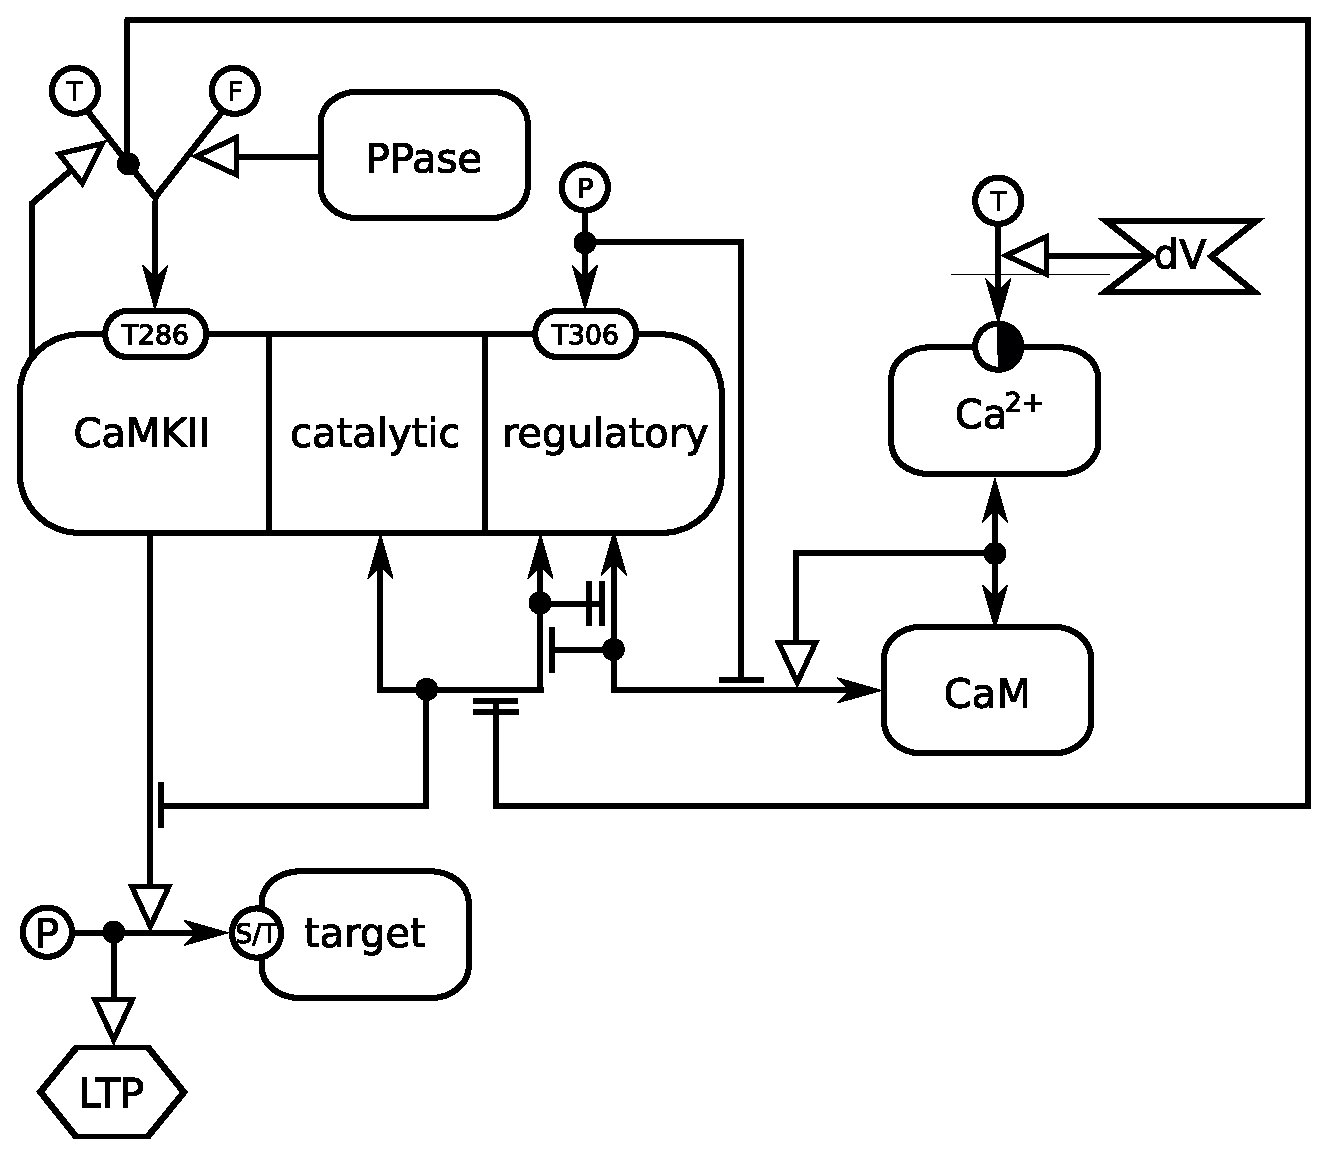
\includegraphics[scale=0.8]{examples/CaMKII-intro}
   \caption{This example of a \ER shows ...}
  \label{fig:eg1}
\end{figure}

The diagram in \fig{eg1} is a simple diagram for ...
 
The essence of the \ER is ... It shows how different entities in the system ... interact ...  

In the example of \fig{eg1}, 

All nodes in \ER

% 
% \tab{component-summary} summarizes the different SBGN abstractions described in this chapter.
% 
% \newcolumntype{P}[1]{>{\raggedright\hspace{0pt}\arraybackslash}p{#1}}
% 
% \begin{table}[bh]
%   \centering
%   \small
%   \begin{tabular}{@{}llP{2.4in}P{1.6in}@{}}
%     \toprule
%     \textbf{Component} & \textbf{Abbrev.} & \textbf{Role} & \textbf{Examples}\\
%     \midrule
%     Entity pool node
%     & EPN
%     & A population of entities that cannot be distinguished from each other
%     & Specific macromolecules or other chemical species \\[0.5em]
% 
%     Container node	
%     & CN
%     & An encapsulation of one or more other SBGN constructs
%     & Complexes, compartments \\[1.6em]
% 
%     Process node
%     & PN
%     & A process that transforms one or more EPNs into one or more other EPNs
%     & Transition, association, dissociation \\[0.5em]
% 
%     Connecting arc
%     & ---
%     & Links between EPNs or CNs to PNs or CNs to indicate influences
%     & Production, catalysis, inhibition \\[0.5em]
% 
%     Logical operators
%     & ---
%     & Combines one or several inputs into one output
%     & Boolean \emph{and}, \emph{or}, \emph{not} \\
%     \bottomrule
%   \end{tabular}
%   \caption{Summary of \PD components and their roles.}
%   \label{tab:component-summary}
% \end{table}

